\begin{ZhChapter}

    \chapter{Methodology}
    In this section, we will introduce the S2GE-NIDS (structured semantics and generation embedded network intrusion detection system) architecture and detail its operational workflow, clearly delineating each step from semantic tokenization through anomaly detection and decision-making processes.
    \section{Architecture} %Chapter 3.1
    The architecture of S2GE-NiDS is presented as Figure \ref{fig:Architecture}, including preprocess model, embedding model, and Mahalanobis model.

    \begin{figure*}[htbp]
        \centering
        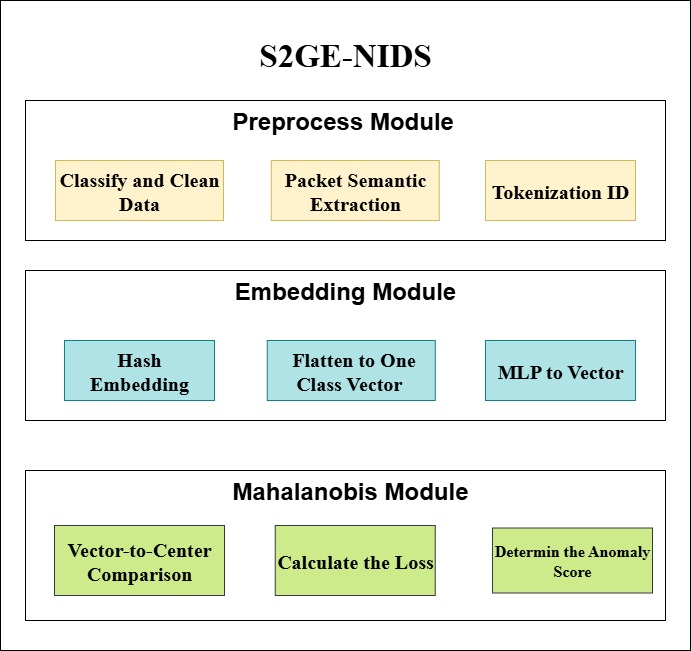
\includegraphics[width = 0.7\textwidth]{image/architecture.png}
        \caption{Architecture of S2GE-NIDS}
        \label{fig:Architecture}
    \end{figure*}

    The further description will begin in the section 3.1.1.

    \subsection{Preprocess Model}
    In the preprocessing phase, we will do the following processes as data file classify and clean, packet semantic extraction, and tokenization. These steps are designed to transform raw network traffic into structured representations suitable for semantic embedding and anomaly detection.

    \subsubsection{Classify and Clean Data}

    The first step in the preprocessing pipeline involves selecting and filtering data files to ensure their suitability for subsequent analysis. In this study, network traffic is collected and stored in the Comma-Separated Values (CSV) format, a widely adopted and flexible tabular data structure. CSV files are particularly well-suited for structured data representation due to their ease of parsing, compact storage, and seamless integration with mainstream data analysis libraries such as pandas and NumPy in Python.

    After selecting the data format, the raw data are merged into a unified DataFrame and subjected to a series of cleaning procedures. First, all column names are normalized by removing extraneous whitespace and converting naming conventions where necessary to ensure consistency across feature dimensions. Next, column values containing missing or undefined entries are removed to prevent bias in downstream training. Finally, columns that contain only zeros are discarded.

    During this stage, the resulting dataset serves as the foundation for the subsequent tokenization and embedding stages.

    \subsubsection{Packet Semantic Extraction}

    Packet semantic extraction refers to the process of identifying and transforming raw packet-level attributes into semantically meaningful representations that facilitate accurate anomaly detection. As summarized in Table~2.1, a set of representative features—such as \textit{Destination Port}, \textit{Protocol Type}, \textit{Flow Duration}, \textit{Packet Length}, \textit{Flow Bytes per Second}, \textit{TCP Flag Counts}, and \textit{Connection Count}—have been consistently validated in prior studies as effective indicators of anomalous or malicious traffic behavior.





    \subsubsection{Tokenization ID}
    Following the feature extraction phase, the structured network traffic attributes undergo a tokenization process, wherein categorical feature fields are transformed into discrete, semantically interpretable string tokens. These tokens form the foundation for subsequent vector embedding. The dataset comprises multiple structured records, each containing various categorical attributes—such as \texttt{Destination Port}, \texttt{Protocol Type}, and \texttt{Source IP Address}—that capture the behavioral characteristics of individual traffic flows. By converting these symbolic fields into tokenized string representations, the model preserves both the identity and contextual meaning of traffic patterns, thereby enabling more effective semantic encoding in later stages.



    Table~\ref{tab:token_example} shows the tokenization method employed, where each feature is transformed by concatenating its field name and corresponding value into a token. For example, \textit{"DestinationPort:80"}, \textit{"FlowDuration:0.32817"}, and \textit{"ProtocolType:TCP"}.

    \begin{table*}[htbp]
        \centering
        \caption{Example of Tokenization}
        \label{tab:token_example}
        \vspace{1em}
        \makebox[\linewidth][c]{
            \renewcommand\arraystretch{1.2}{
                \begin{tabular}{| l | l | l |}
                    \hline
                    \textbf{Field Name} & \textbf{Field Value} & \textbf{Token}       \\
                    \hline
                    Destination Port    & 80                   & DestinationPort:80   \\
                    Flow Duration       & 0.32817              & FlowDuration:0.32817 \\
                    Protocol Type       & TCP                  & ProtocolType:TCP     \\
                    \hline
                \end{tabular}
            }}
    \end{table*}



    \subsection{Embedding Model} %3.1.2
    To convert network packet features into vector representations that can be processed by the model, this architecture employs an efficient embedding model. The entire process includes Hash Embedding, flattening to a one-class vector, and using a multilayer perceptron (MLP) to vector.



    \subsubsection{Hash Embedding} %3.1.2.1
    Hash embedding is a lightweight vectorization technique that utilizes non-cryptographic hashing to encode tokenized field-value pairs into fixed-size, trainable embeddings. In this study, we adopt the MurmurHash3 algorithm, an efficient and widely used hash function, to map each token to a specific position in the embedding table. Its advantages include fast computation, uniform distribution, and language-independent implementation, making it well-suited for scalable anomaly detection in IoT environments.

    To determine the target index for each token, we apply a modulo operation to the hash value using the smallest three-digit prime number, 233. This approach distributes tokens more evenly within the embedding space and reduces collision rates.

    Figure~\ref{fig:EmbeddingFlow} presents a representative subset of the embedding table used in our model, where each token derived from structured field-value pairs is mapped to an index through hashing and modulo operations.

    In this process, both field names and their corresponding values are individually hashed using the MurmurHash3 function. The resulting integers are then projected into a fixed index range via modulo operation with a prime number \(P=233\), producing bounded coordinates in the embedding table. For instance as Figure~\ref{fig:hashembedding}, the field name \texttt{Destination\_Port} yields an index of 129, while its value \texttt{80} maps to 166; these indices are used to locate specific embedding vectors.

    Each vector is initialized randomly and refined during model training. The retrieved embeddings, such as the example 8-dimensional vector for indices (166, 129), capture semantic properties of the original tokens and are later concatenated as input to the MLP encoder for higher-level representation learning.

    \begin{figure*}[htbp]
        \centering
        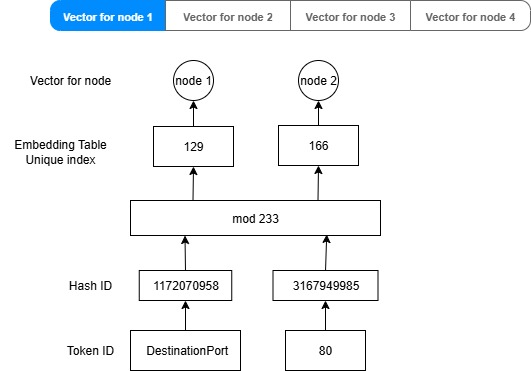
\includegraphics[width = 0.7\textwidth]{image/EmbeddingFlow.jpg}
        \caption{Hash Embedding for Embedding Model}
        \label{fig:EmbeddingFlow}
    \end{figure*}




    \begin{figure*}[htbp]
        \centering
        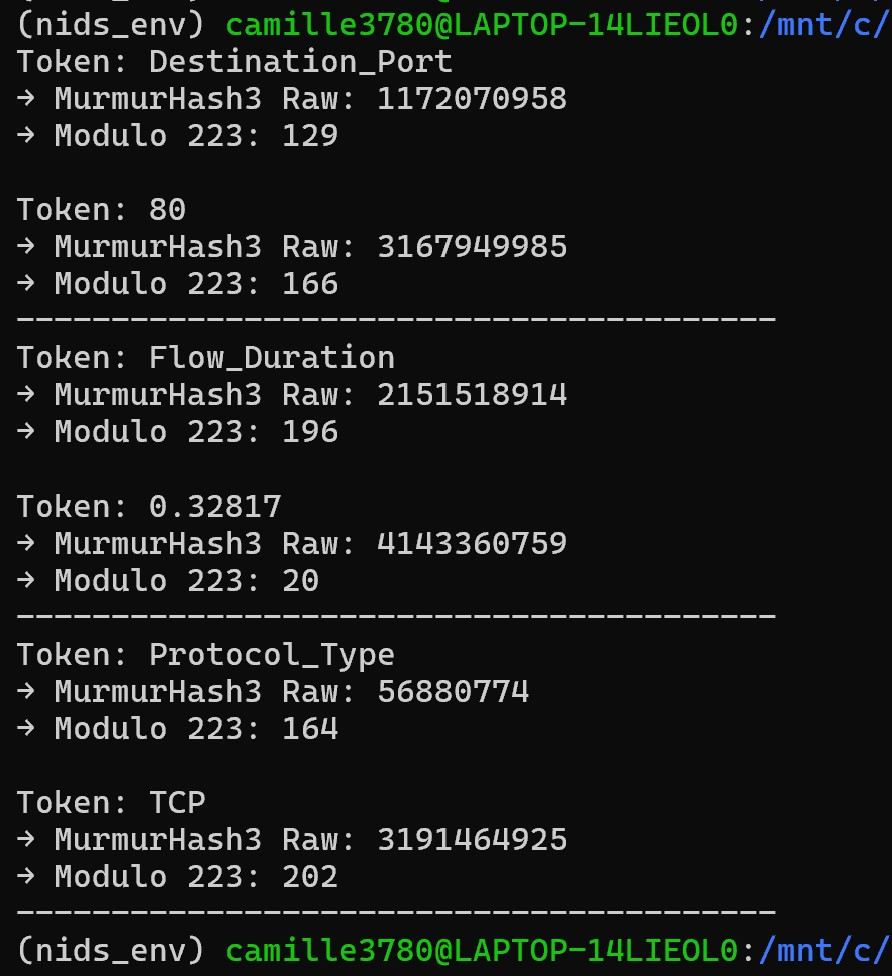
\includegraphics[width = 0.4\textwidth]{image/2025-06-30 002218.jpg}
        \caption{HashEmbedding Process}
        \label{fig:hashembedding}
    \end{figure*}





    \newpage
    \subsubsection{Flatten to One Class Vector}
    The flatten operation concatenates the tokenized embeddings from each column into a single vector for input to the next stage of the pipeline. Table~\ref{tab:token_embedding_table} shows example embedding vectors for individual tokens, such as \texttt{Destination Port} 80 represented by [0.5012, 0.7061, 0.7705, 0.6871, 0.4636, 0.4809, 0.1913, 0.8319], \texttt{Flow Duration} 0.32817 represented by [0.227, 0.9268, 0.676, 0.9304, 0.5891, 0.3531, 0.2451, 0.9082], and \texttt{Protocol} TCP represented by [0.2309, 0.8674, 0.3565, 0.8259, 0.1846, 0.4375, 0.2524, 0.3008]. The final flattened vector is formed by concatenating these embeddings into a single vector is [0.5012, 0.7061, 0.7705, 0.6871, 0.4636, 0.4809, 0.1913, 0.8319, 0.227, 0.9268, 0.676, 0.9304, 0.5891, 0.3531, 0.2451, 0.9082, 0.2309, 0.8674, 0.3565, 0.8259, 0.1846, 0.4375, 0.2524, 0.3008].



    \begin{table}[htbp]
        \scriptsize
        \renewcommand{\arraystretch}{1.2}
        \caption{HashValue of Embedding Table Value}
        \vspace{1em}
        \begin{tabular}{| c | c | c |l|}
            \hline
            \textbf{Token}    & \textbf{Hash} & \textbf{Mod=223} & \textbf{Embedding Vector}                                        \\
            \hline
            Destination\_Port & 1172070958    & 129              & [0.5012, 0.7061, 0.7705, 0.6871, 0.4636, 0.4809, 0.1913, 0.8319] \\
            80                & 3167949985    & 166              &                                                                  \\
            \hline
            Flow\_Duration    & 2151518914    & 196              & [0.227, 0.9268, 0.676, 0.9304, 0.5891, 0.3531, 0.2451, 0.9082]   \\
            0.32817           & 4143360759    & 20               &                                                                  \\
            \hline
            Protocol\_Type    & 56880774      & 164              & [0.2309, 0.8674, 0.3565, 0.8259, 0.1846, 0.4375, 0.2524, 0.3008] \\
            TCP               & 3191464925    & 202              &                                                                  \\
            \hline
        \end{tabular}
        \label{tab:token_embedding_table}
    \end{table}





    \subsubsection{MLP to Vector}
    To integrate the multiple field semantic vectors extracted from the embedding table for each packet into a unified semantic representation, a multi-layer perceptron (MLP) encoder module is introduced. The main task of this module is to map a flattened one-dimensional vector \(\mathbf{x} \in \mathbb{R}^{F \times d}\) to a fixed-dimensional semantic feature vector \(\mathbf{z} \in \mathbb{R}^k\), where \(F\) is the number of fields, \(d\) is the embedding dimension of each field, and \(k\) is the dimension of the output vector.

    In order to integrate multiple semantic vectors extracted from the embedding table for each field into a unified semantic representation, we designed a multi-layer perceptron (MLP) encoding module. The input layer accepts a flattened vector \(F\), where \(F\) is the number of fields and \(d\) is the dimension of the embedding vector for each field. This vector will be mapped to a fixed-dimensional semantic feature vector \(\mathbf{z} \in \mathbb{R}^k\), Where \(k\) is the dimension of the output sense vector.

    The MLP is composed of multiple fully connected layers as in Figure~\ref{fig:MLP}.


    \begin{figure*}[htbp]
        \centering
        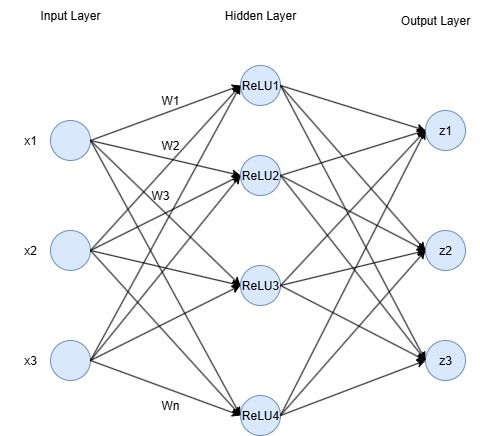
\includegraphics[width = 0.6\textwidth]{image/MLP.jpg}
        \caption{Multilayer Perceptron architecture the full connection and ReLU activation from input layer to hidden layer to output layer}
        \label{fig:MLP}
    \end{figure*}


    \subsection{Mahalanobis Distance Model}
    In the final stage of the S2GE-NIDS framework, a statistical distance-based method—\textbf{Mahalanobis Distance}—is applied to evaluate whether an observed semantic vector deviates significantly from the expected distribution of normal traffic. This metric is particularly effective for high-dimensional anomaly detection, as it accounts for feature correlations and variance~\cite{de2000mahalanobis}.





    \subsubsection{Vector-to-Center Comparison}
    To enhance anomaly detection, S2GE-NIDS incorporates a center loss mechanism. During training, all semantic vectors corresponding to ``normal'' samples are aggregated to compute a center point \(c\).



    By accounting for the variability and correlation of each feature, the model is able to more accurately detect abnormal samples that are ``off-center.''




    \begin{equation}
        D_M(z) = \sqrt{(z - c)^T \Sigma^{-1} (z - c)} \tag*{\makebox[3.8cm][r]{\cite{mahalanobis1936generalized}}}
        \label{eq:mahalanobiseq}
    \end{equation}

    $z$ is the semantic vector of the input sample, $c$ is the center vector of normal samples, and $\Sigma^{-1}$ is the inverse of the covariance matrix of the training data's embedding vectors.


    \subsubsection{Calculate the Loss}
    \begin{itemize}
        \item The loss is defined as:
    \end{itemize}

    \begin{equation}
        \mathcal{L} = \frac{1}{N} \sum_{i=1}^{N} \| z_i - c \|^2
        = \frac{1}{N} \sum_{i=1}^{N} \sum_{j=1}^{d} (z_{ij} - c_j)^2 \tag*{\makebox[3.8cm][r]{\cite{mlp2001universal}}}
        \label{eq:centerloss}
    \end{equation}

    $z_i \in \mathbb{R}^d$ is the embedding vector obtained after the $i$th input passes through the Semantic Encoder,
    $c \in \mathbb{R}^d$ is the center point vector during training (center), and $N$ is the total number of samples.



    \subsubsection{Determine the Anomaly Score}
    After obtaining the semantic vector \(\mathbf{z}\) of each input data point through the MLP encoder, and computing the center point \(\mathbf{c}\) based on all normal training samples, the system evaluates how far each sample deviates from the normal data distribution using the Mahalanobis distance metric.

    The Mahalanobis distance score \(D_M(\mathbf{z})\), quantifies the distance between a sample's semantic representation \(\mathbf{z}\) and the center vector \(\mathbf{c}\), while accounting for the variance and covariance of the embedding space. This distance serves as the anomaly score for each sample.

    To determine whether a sample is anomalous, a threshold \(\tau\) is defined based on the distribution of distances observed in the training data. A sample is classified as anomalous if its Mahalanobis distance exceeds this threshold:

    \begin{equation}
        \text{Anomaly}(z) =
        \begin{cases}
            1 & \text{if } D_M(z) > \tau                                            \\
            0 & \text{otherwise} \tag*{\makebox[3.8cm][r]{\cite{mlp2001universal}}}
        \end{cases}
    \end{equation}

    This threshold-based mechanism enables the system to make binary decisions (normal vs. anomalous) while preserving the interpretability and statistical grounding of the anomaly scores.





    \section{Flow} %Chapter 3.2
    This section presents the flow of proposed system. The complete workflow consists of three main components: the Preprocessing Model, the Embedding Model, and the Mahalanobis Distance model.

    \subsection{Preprocess Model}
    As shown in Figure~\ref{fig:FlowChart}, the system receives the uploaded network packet data and verifies whether its format conforms to the CSV (Comma-Separated Values) format. We using Pandas and NumPy to data selection and cleaning stage. This includes standardizing column names, removing missing or undefined values, and deleting columns that contain only zeros to reduce noise.




    \begin{figure*}[htbp]
        \centering
        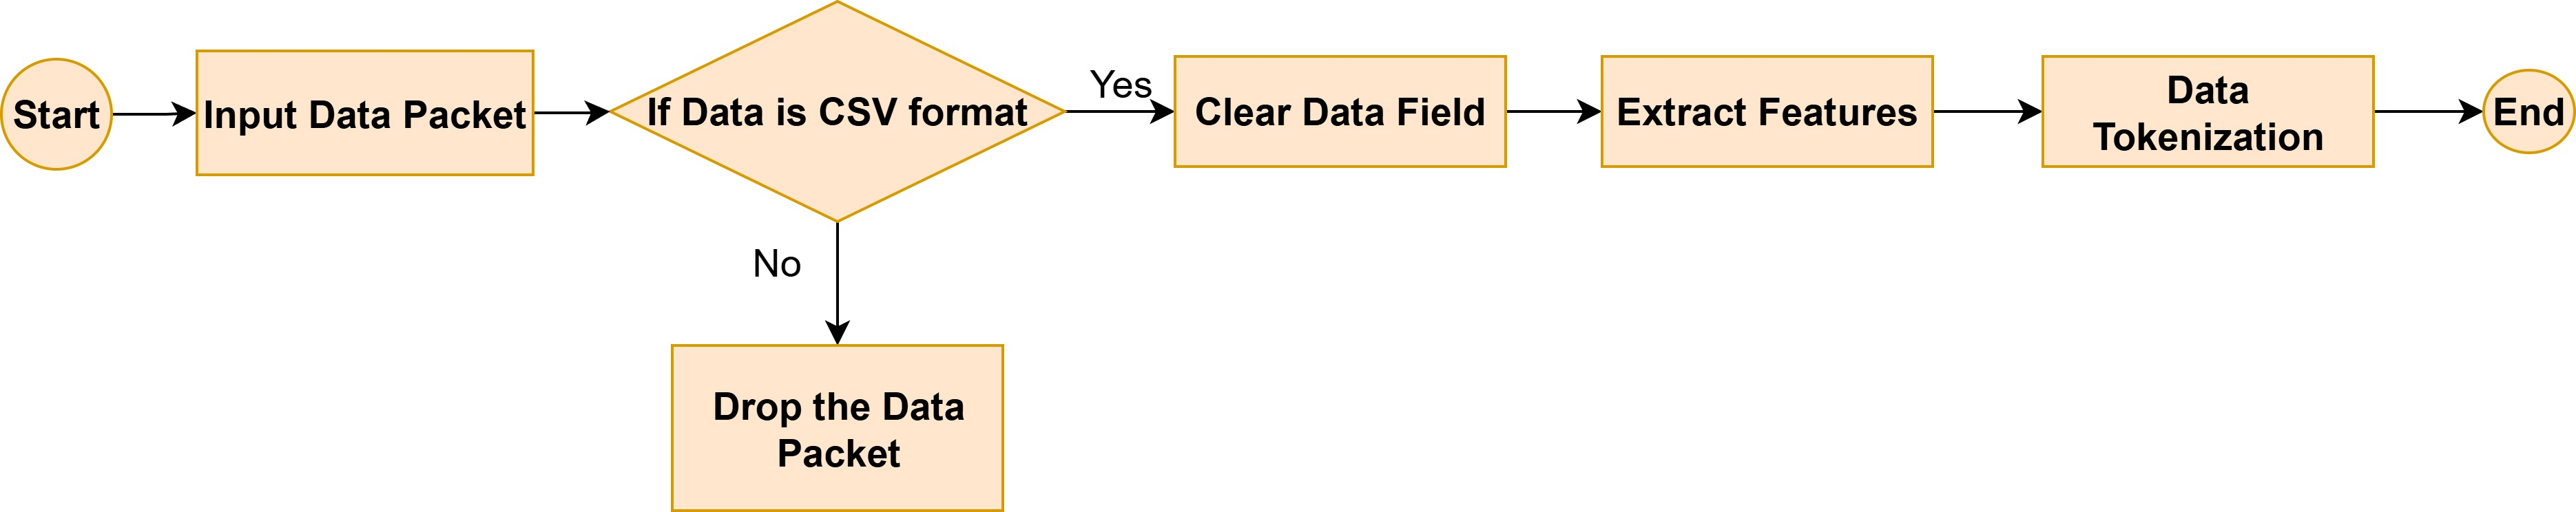
\includegraphics[width = 1\textwidth]{image/FlowChart.jpg}
        \caption{Process for Preprocess Model}
        \label{fig:FlowChart}
    \end{figure*}

    We use specific fields related to common anomaly detection features are extracted, such as \texttt{Destination Port}, \texttt{Protocol Type}, and \texttt{Source IP} (\texttt{SrcIP}). These fields serve as important inputs for subsequent model analysis.

    Then, the field names and their respective values are combined into tokens—for example, \texttt{Protocol\_TCP} or \texttt{Port\_80}—and fed into a semantic embedding model to be transformed into vectors for further processing.




    \subsection{Embedding Model}
    In Figure~\ref{fig:hashembeddingflow}, this module is responsible for converting the structured semantic token sequence into a fixed-dimensional numerical vector representation. This module includes Hash Embedding, Flatten to One Class Vector, and MLP to Vector. Each of them contributes to the lightweight and scalable nature of the system.

    \begin{figure*}[htbp]
        \centering
        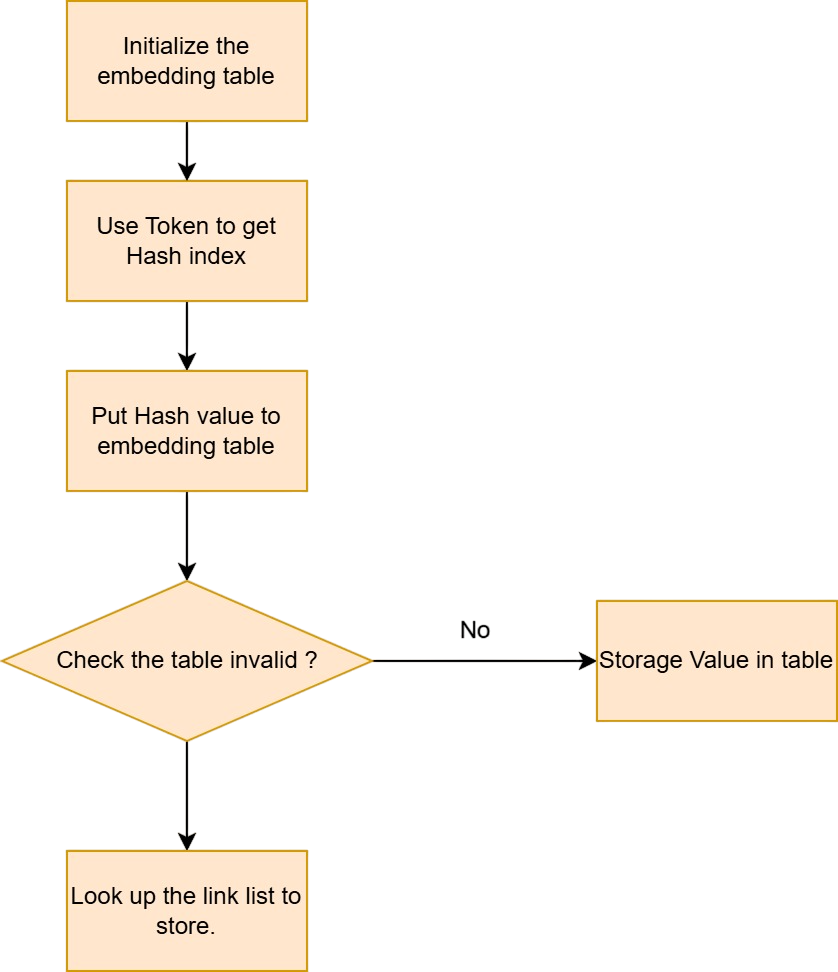
\includegraphics[width = 1\textwidth]{image/hashembedding.jpg}
        \caption{Hash Embedding for Embedding Model}
        \label{fig:hashembeddingflow}
    \end{figure*}

    Traditional one-hot or dictionary embedding methods require maintaining a vocabulary, which is inefficient for IoT packet data. Therefore, this study employs the non-cryptographic hash function MurmurHash3 to map each \texttt{<field name>:<value>} token to a trainable embedding position.

    To map discrete feature tokens into a fixed-size embedding space without maintaining a predefined vocabulary, a dual-stage hash embedding strategy is utilized. Each token in the form of \texttt{<FieldName>:<Value>} is decomposed into two components: the field identifier and the associated value. Both components are independently processed by the MurmurHash3 function, which offers fast computation and near-uniform distribution.

    Formally, for a given token $t = \texttt{Field:Value}$, we compute:

    \begin{equation}
        \text{row\_idx} = \text{MurmurHash3}(\texttt{Field}) \bmod P
    \end{equation}

    \begin{equation}
        \text{col\_idx} = \text{MurmurHash3}(\texttt{Value}) \bmod P
    \end{equation}

    where $P = 233$ is a small prime number chosen to reduce the probability of hash collisions and to ensure efficient modular indexing.

    The resulting $(\text{row\_idx}, \text{col\_idx})$ pair identifies a unique coordinate in the 2D embedding table $\mathbf{E} \in \mathbb{R}^{P \times P \times d}$, where each entry holds a trainable $d$-dimensional embedding vector.


    Parameter Learning and Training Process of the MLP

    In the proposed S2GE-NIDS system, the Multilayer Perceptron (MLP) sparse embedding vectors into low-dimensional continuous semantic representations. The MLP parameters, including weight matrices and bias vectors, are not manually set but are learned automatically during the neural network training process. The following details this process:


    Parameter Initialization: At the beginning of training, all weight matrices $\mathbf{W}_i$ and bias vectors $\mathbf{b}_i$ are initialized randomly. Common initialization techniques, such as Xavier initialization \cite{glorot2010understanding}, ensure that gradients maintain appropriate scale to prevent vanishing during training.

    Forward Propagation

    Given an input vector $\mathbf{X} \in \mathbb{R}^{d_{\text{in}}}$, the MLP performs a series of linear transformations and nonlinear activations layer by layer, computing:


    \begin{align}
        \mathbf{H}_1 & = \sigma(\mathbf{W}_1 \mathbf{X} + \mathbf{b}_1)   \\
        \mathbf{H}_2 & = \sigma(\mathbf{W}_2 \mathbf{H}_1 + \mathbf{b}_2) \\
                     & \vdots \nonumber                                   \\
        \mathbf{Z}   & = \mathbf{W}_L \mathbf{H}_{L-1} + \mathbf{b}_L
    \end{align}

    where $\sigma(\cdot)$ is typically the ReLU activation function defined as:

    \begin{equation}
        \mathrm{ReLU}(z) = \max(0, z)
    \end{equation}

    and $\mathbf{Z} \in \mathbb{R}^k$ represents the output semantic vector.

    Loss Function Computation: During training, a loss function $\mathcal{L}$ measures the discrepancy between the model output and the target. For example, using a center loss \cite{wen2016discriminative} to encourage semantic vectors of normal samples to cluster around a center $\mathbf{c}$:


    \begin{equation}
        \mathcal{L} = \frac{1}{N} \sum_{i=1}^N \| \mathbf{z}_i - \mathbf{c} \|^2
    \end{equation}

    Iterative Training: This process is repeated over multiple epochs on the training dataset. Through iterative updates, the model gradually minimizes the loss, improving its ability to distinguish normal and anomalous samples.

    給一個總結



    \subsection{Mahalanobis Distance Model}
    In this section, we present an anomaly detection method based on the Mahalanobis distance as the core model for decision making. The discussion is organized into three parts: Vector-to-Center Comparison, Calculate the Loss, and Determin the Anomaly Score.
    注重flow,不是架構

    Given $N$ semantic vectors $\mathbf{z}_1, \dots, \mathbf{z}_N$ generated from benign training data, we first compute the statistical mean (center) vector $\boldsymbol{c}$ and covariance matrix $\boldsymbol{\Sigma}$:

    \begin{equation}
        \boldsymbol{c} = \frac{1}{N} \sum_{i=1}^{N} \mathbf{z}_i
    \end{equation}

    \begin{equation}
        \boldsymbol{\Sigma} = \frac{1}{N - 1} \sum_{i=1}^{N} (\mathbf{z}_i - \boldsymbol{c})(\mathbf{z}_i - \boldsymbol{c})^T
    \end{equation}



    For any test vector $\mathbf{z}$, the Mahalanobis distance $D_M(\mathbf{z})$ from the normal distribution is calculated as:

    \begin{equation}
        D_M(\mathbf{z}) = \sqrt{(\mathbf{z} - \boldsymbol{c})^T \boldsymbol{\Sigma}^{-1} (\mathbf{z} - \boldsymbol{c})}
    \end{equation}

    A larger distance indicates a greater deviation from the normal behavior, suggesting a higher probability of being anomalous.



    We define a threshold $\tau$ based on the distribution of $D_M(\cdot)$ in the training data (e.g., 95th percentile).

    \begin{equation}
        \text{Anomaly}(\mathbf{z}) =
        \begin{cases}
            1, & \text{if } D_M(\mathbf{z}) > \tau \\
            0, & \text{otherwise}
        \end{cases}
    \end{equation}



    \begin{itemize}
        \item \textbf{Input}: Semantic vector $\mathbf{z} \in \mathbb{R}^k$ (from MLP)
        \item \textbf{Output}: Anomaly score $D_M(\mathbf{z})$ and binary decision
        \item \textbf{Computation}: Based on $\boldsymbol{c}$ and $\boldsymbol{\Sigma}$ estimated from training data
    \end{itemize}



    \begin{itemize}
        \item \textbf{Unsupervised}: Requires only benign data for training
        \item \textbf{Interpretable}: Outputs a clear statistical distance as anomaly score
        \item \textbf{Statistically Sound}: Incorporates feature correlation via covariance
        \item \textbf{Efficient}: Only requires mean and covariance estimation once during training
    \end{itemize}


    總結: 1就是異常,0就是正常

\end{ZhChapter}